\documentclass[slidestop,mathserif,compress,xcolor=svgnames]{beamer} 
\mode<presentation>
{  
  \setbeamertemplate{background canvas}[vertical shading][bottom=blue!5,top=blue!5]
  \setbeamertemplate{navigation symbols}{}%{\insertsectionnavigationsymbol}
  \usetheme{LSU}
%  default infolines miniframes shadow sidebar smoothbars smoothtree split tree
%    \useoutertheme{shadow}
}

\usepackage{pgf,pgfarrows,pgfnodes,pgfautomata,pgfheaps,pgfshade}
\usepackage{amsmath,amssymb,amsfonts,subfigure}
\usepackage{multirow,rotating}
\usepackage{tabularx}
\usepackage{booktabs}
\usepackage{colortbl}

\usepackage[english]{babel}
\usepackage[latin1]{inputenc}
\usepackage[T1]{fontenc}
\usepackage{times}
\usepackage[normalem]{ulem}
\usepackage{graphicx}
\usefonttheme{serif}

\usepackage{tikz}
\usetikzlibrary{shapes,arrows}
\usetikzlibrary{calc}
\pgfdeclarelayer{background}
\pgfdeclarelayer{foreground}
\pgfsetlayers{background,main,foreground}

\usepackage{hyperref}
% \usepackage{movie15}
\hypersetup{
  pdftitle={Introduction to GNU Octave},
  pdfauthor={Alexander B. Pacheco, User Services Consultant, Louisiana State University}
}
%\usepackage{movie15}
\usepackage{times}

\setbeamercovered{dynamic}
\beamersetaveragebackground{DarkBlue!2}
\beamertemplateballitem

\definecolor{DarkGreen}{rgb}{0.0,0.3,0.0}
\definecolor{darkgreen}{rgb}{0.0,0.6,0.0}
\definecolor{Blue}{rgb}{0.0,0.0,0.8} 
\definecolor{dodgerblue}{rgb}{0.1,0.1,1.0}
\definecolor{indigo}{rgb}{0.41,0.1,0.0}
\definecolor{seagreen}{rgb}{0.1,1.0,0.1}
\DeclareSymbolFont{extraup}{U}{zavm}{m}{n}
\DeclareMathSymbol{\vardiamond}{\mathalpha}{extraup}{87}
\newcommand*\up{\textcolor{green}{%
  \ensuremath{\blacktriangle}}}
\newcommand*\down{\textcolor{red}{%
  \ensuremath{\blacktriangledown}}}
\newcommand*\const{\textcolor{darkgray}%
  {\textbf{--}}}
\newcommand{\bftt}[1]{\textbf{\texttt{#1}}}

\setbeamercolor{uppercol}{fg=white,bg=red!30!black}%
\setbeamercolor{lowercol}{fg=black,bg=red!15!white}%
\setbeamercolor{uppercol1}{fg=white,bg=blue!30!black}%
\setbeamercolor{lowercol1}{fg=black,bg=blue!15!white}%%
\setbeamercolor{uppercol2}{fg=white,bg=green!30!black}%
\setbeamercolor{lowercol2}{fg=black,bg=green!15!white}%
\setbeamercolor{uppercol3}{fg=white,bg=green!50!red!50!black}%
\setbeamercolor{lowercol3}{fg=black,bg=green!60!red!30!white}%
\setbeamercolor{uppercol4}{fg=white,bg=green!30!blue!50!black}%
\setbeamercolor{lowercol4}{fg=black,bg=green!30!blue!50!white}%
\newenvironment{ablock}[0]
{
\begin{beamerboxesrounded}[upper=uppercol,lower=lowercol,shadow=true]}
{\end{beamerboxesrounded}}
\newenvironment{bblock}[0]
{
\begin{beamerboxesrounded}[upper=uppercol1,lower=lowercol1,shadow=true]}
{\end{beamerboxesrounded}}
\newenvironment{eblock}[0]
{
\begin{beamerboxesrounded}[upper=uppercol2,lower=lowercol2,shadow=true]}
{\end{beamerboxesrounded}}
\newenvironment{beblock}[0]
{
\begin{beamerboxesrounded}[upper=uppercol3,lower=lowercol3,shadow=true]}
{\end{beamerboxesrounded}}
\newenvironment{eeblock}[0]
{
\begin{beamerboxesrounded}[upper=uppercol4,lower=lowercol4,shadow=true]}
{\end{beamerboxesrounded}}

% Fix font size of nested itemize/enumerate
\setbeamerfont{itemize/enumerate body}{}
\setbeamerfont{itemize/enumerate subbody}{size=\scriptsize}
\setbeamerfont{itemize/enumerate subsubbody}{size=\scriptsize}

\title[GNU Octave]{Introduction to GNU Octave}


\author[Alex Pacheco]{\large{Alexander~B.~Pacheco}}
       
\institute[HPC@LSU - http://www.hpc.lsu.edu] {\inst{}\footnotesize{User Services Consultant\\LSU HPC \& LONI\\sys-help@loni.org}}

\date[{Apr. 18, 2012\hspace{2cm}}]{\scriptsize{HPC Training Series\\Louisiana State University\\Baton Rouge\\Apr. 18, 2012}}
     
\subject{Talks}
% This is only inserted into the PDF information catalog. Can be left
% out. 




% If you have a file called "university-logo-filename.xxx", where xxx
% is a graphic format that can be processed by latex or pdflatex,
% resp., then you can add a logo as follows:

% Main Logo on bottom left
\pgfdeclareimage[height=0.55cm]{its-logo}{LONI}
\logo{\pgfuseimage{its-logo}}
% University Logo on top left
\pgfdeclareimage[height=0.55cm]{university-logo}{LSUGeauxPurp}
\tllogo{\pgfuseimage{university-logo}}
% Logo at top right
\pgfdeclareimage[height=0.6cm]{institute-logo}{PUR_BLK_HOR}
\trlogo{\pgfuseimage{institute-logo}}
% Logo at bottom right
\pgfdeclareimage[height=0.55cm]{hpc-logo}{CCT}
\brlogo{\pgfuseimage{hpc-logo}}


% Delete this, if you do not want the table of contents to pop up at
% the beginning of each subsection:
  \AtBeginSection[]
  {
    \begin{frame}<beamer>
     \frametitle{\small{Outline}}
      \small
      \tableofcontents[currentsection,currentsubsection]
    \end{frame}
  }

\begin{document}
\scriptsize

\frame{\titlepage}

\begin{frame}[label=toc,squeeze]
  \footnotesize
  \frametitle{\small{Outline}}
  \tableofcontents
\end{frame}

\section{Introduction}
\begin{frame}
  \frametitle{\small What is GNU Octave?}
  \begin{itemize}
    \item Octave is a high-level language, primarily intended for numerical computations. 
    \item It provides a convenient command line interface for solving linear and nonlinear problems numerically, and for performing other numerical experiments. 
      \item It may also be used as a batch-oriented language.
      \item Octave is often viewed as a system for numerical computations with a language that is mostly compatible with Matlab, but that is available as free software under the GNU GPL, and that can replace it in many circumstances.
  \end{itemize}

  \begin{eblock}{Tutorial Goals}
    \begin{itemize}
      \item The goal of this tutorial is to provide a brief introduction to a few of the capabilities of GNU Octave.
      \item Most of the functionality of Matlab already exists in GNU Octave and octave can run most Matlab scripts.
      \item Matlab users should review differences between Matlab and GNU Octave before porting matlab scripts to octave. \url{http://en.wikibooks.org/wiki/MATLAB_Programming/Differences_between_Octave_and_MATLAB}
    \end{itemize}
  \end{eblock}
\end{frame}

\begin{frame}
  \frametitle{\small Requirements}
  \begin{itemize}
    \item Users can install GNU Octave on their laptops and desktops.
    \item{Mac OS X:} \url{http://www.octave.org/wiki/index.php?title=Installing_MacOS_X_Bundle}
    \item{Windows:} \url{http://www.octave.org/wiki/index.php?title=Octave_for_Windows} 
    \item{Linux:} Check repositories for your distribution
    \begin{enumerate}
      \item{openSuSE:} \texttt{zypper in octave}
      \item{Ubuntu:} \texttt{apt-get install octave}
      \item{Fedora:} \texttt{yum install octave}
    \end{enumerate}
    \item LSU HPC \& LONI: Add soft key +octave-3.0.3-intel-11.1 to your .soft file and resoft
  \end{itemize}
\end{frame}

\section{Getting Started}
\begin{frame}%[allowframebreaks]
  \frametitle{\small Getting Started}
  \begin{itemize}
    \item Type \texttt{octave} in a terminal window (Linux, LSU HPC \& LONI only)
  \end{itemize}
  \begin{center}
    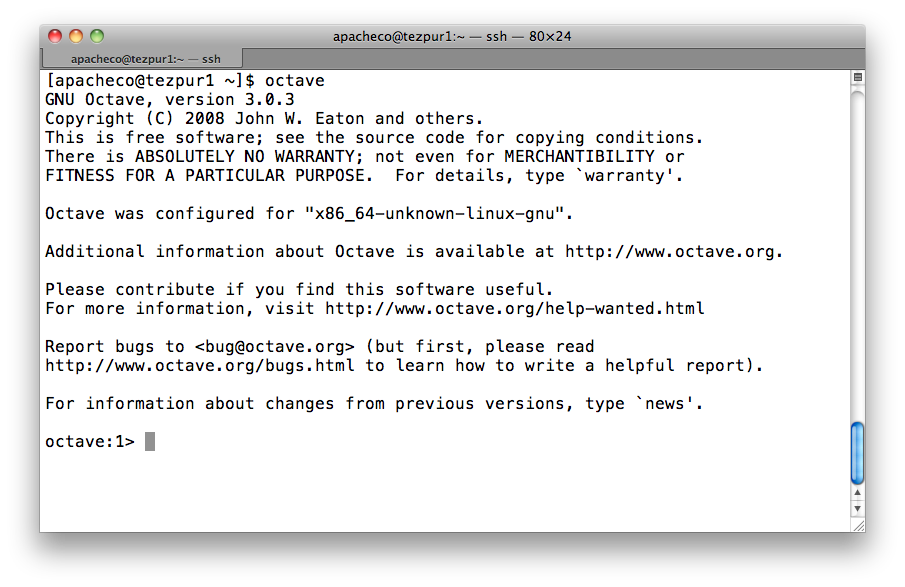
\includegraphics[width=0.75\textwidth,clip=true]{octave-startup}
  \end{center}
  \begin{itemize}
    \item The last line is the octave prompt
    \item You can also start octave with the -q option, octave information will not be printed
  \end{itemize}
\end{frame}

\begin{frame}[allowframebreaks]
  \frametitle{\small Entering Commands}
  \begin{itemize}
    \item Commands can be typed at the prompt or read from a script.
    \item Scripts are plain text files with file suffix \texttt{.m}.
    \item To run a script, type the script name without the suffix.
    \item ``,'' separates commands in a line and displays the output on the screen.
    \item To suppress output, use ``;''.
    \item Comments are preceeded by \%.
    \item Octave is case-sensitive.
    \item Getting Help:
    \begin{itemize}
      \item \texttt{help} lists all built-in functions and internal variables.
      \item \texttt{help name} explains the variable or function "name"
    \end{itemize}
    \framebreak
    \item Octave as a calculator:
    \begin{itemize}
      \item Just type mathematical commands at the prompt.
      \item Octave also has mathematical built-in functions.
    \end{itemize}
  \end{itemize}
  \begin{columns}
    \column{0.3\textwidth}
    \begin{eblock}{Simple Arithmetic functions}
      \begin{description}
        \item[Addition:] +
        \item[Subtraction:] -
        \item[Multiplication:] *
        \item[Division:] /
        \item[Exponentiation:] **
      \end{description}
    \end{eblock}
    \column{0.6\textwidth}
    \begin{eblock}{Mathematical Functions}
      \begin{description}
        \item[Trignometic Functions:] sin, cos, tan
        \item[Inverse Trignometric Functions:] asin, acos, atan
        \item[Logarithmic Functions:] log, log10
        \item[Exponentiation:] exp
        \item[Absolute value:] abs
      \end{description}
    \end{eblock}
  \end{columns}
  \begin{itemize}
    \item trignometric functions work in \textbf{radians}
    \item \textbf{pi, e, i} and \textbf{j} are predefined variables.
    \item \textbf{ans} variable is used to hold the result of the last operation.
    \item No need to declare variable or its type, variables are either \textbf{floating point} numbers or \textbf{strings}.
    \item To see the value of a variable, just type its name and hit return.
    \begin{center}
      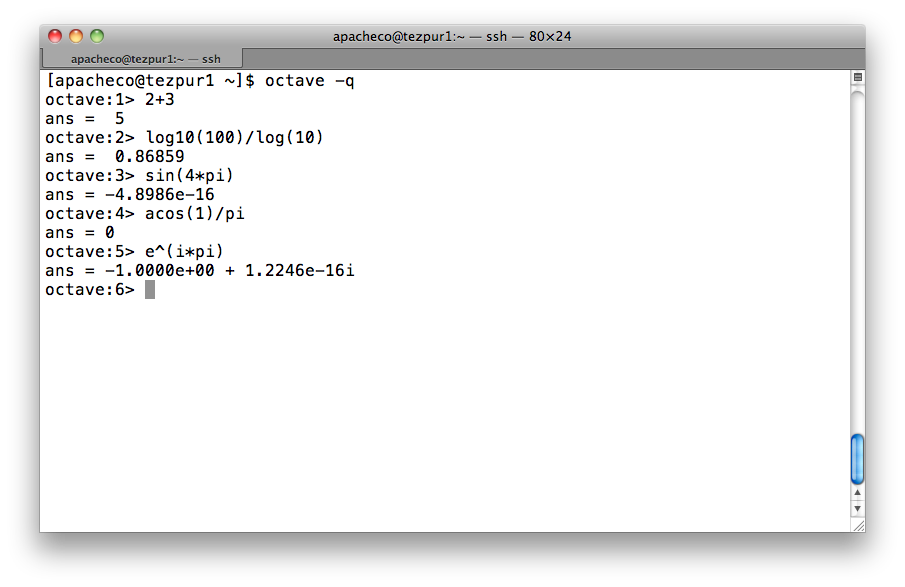
\includegraphics[width=0.75\textwidth,clip=true]{octave-simple}
    \end{center}
    \item Note that by default, octave prints variables with only 5 digits.
    \item At octave prompt, type \texttt{format long} to obtain variables with greater precision.
  \end{itemize}
\end{frame}

\section{Vectors and Matrices}
\begin{frame}[fragile]
  \frametitle{\small Vectors}
  \begin{itemize}
    \item Defining a Row Vector: $vr = (1\,2\,3)$
    \begin{verbatim}
octave:1> vr = [1 2 3]
vr =

   1   2   3
    \end{verbatim}
    \item Defining a Column Vector: $vc = (vr)^T$ 
    \begin{verbatim}
octave:2> vc = [1; 2; 3]
vc =

   1
   2
   3
    \end{verbatim}
    \item Autogeneration of Vector with constant increment: \texttt{Start:[increment]:End}
    \begin{verbatim}
octave:3> a = 4:2:10
a =

   4   6   8  10
    \end{verbatim}
  \end{itemize}
\end{frame}

\begin{frame}[fragile,allowframebreaks]
  \frametitle{\small Matrices}
  \begin{itemize}
    \item A matrix $B=\left(\begin{array}{cc}1 & 2 \\ 3 & 4 \end{array}\right)$ is constructed as follows
    \begin{verbatim}
octave:4> B = [1 2; 3 4]
B =

   1   2
   3   4
    \end{verbatim}
    \item Matrices can be assembled from submatrices
    \begin{verbatim}
octave:5> b = 5:6
b =

  5  6
octave:6> A = [ B b']
A =

   1   2   5
   3   4   6
    \end{verbatim}
    \framebreak
    \item Creating special matrices of size $m\times n$
    \begin{enumerate}
      \item eye(m,n): Create a matrix with ones on the diagonal and zeros elsewhere. Identity matrix if $m=n$
      \item zeros(m,n): Create a null matrix
      \item ones(m,n): Create a matrix where all elements are 1
      \item rand(m,n): generates a random matrix whose entries are uniformly distributed in the interval (0,1).
    \end{enumerate}
    {\tiny
    \begin{columns}
      \column{4cm}
      \begin{verbatim}
octave:7> eye(3,2)
ans =

   1   0
   0   1
   0   0

octave:8> eye(3,3)
ans =

   1   0   0
   0   1   0
   0   0   1

octave:9> zeros(3,2)
ans =

   0   0
   0   0
   0   0
      \end{verbatim}
      \column{4cm}
      \begin{verbatim}
octave:10> ones(3,4)
ans =

   1   1   1   1
   1   1   1   1
   1   1   1   1

octave:11> rand(5,2)
ans =

   1.7700e-01   1.4495e-01
   7.5533e-01   7.9854e-01
   3.4831e-04   7.6881e-01
   5.6224e-01   1.0213e-01
   5.3236e-01   9.2427e-01
      \end{verbatim}
    \end{columns}
    }
    \item Basis Arithmetic:
    \begin{itemize}
      \item \texttt{+, - and *} denote matrix addition, subtraction and multiplication respectively.
      \item \texttt{A'}: transpose and conjugates A
      \item \texttt{A.'}: transposes A
    \end{itemize}
    {\tiny
      \begin{columns}
        \column{4cm}
        \begin{verbatim}
octave:1> A = [1+i 2+2i;3-i 4-2i]
A =

   1 + 1i   2 + 2i
   3 - 1i   4 - 2i
octave:3> A+B,A*B
ans =

   3 + 1i   4 + 2i
   5 - 1i   6 - 2i

ans =

    6 +  6i    6 +  6i
   14 -  6i   14 -  6i
        \end{verbatim}
        \column{4cm}
        \begin{verbatim}
octave:2> B = 2*ones(2,2) 
B =

   2   2
   2   2

octave:4> A',A.'
ans =

   1 - 1i   3 + 1i
   2 - 2i   4 + 2i

ans =

   1 + 1i   3 - 1i
   2 + 2i   4 - 2i
        \end{verbatim}
      \end{columns}
    }
    \framebreak
    \item Element wise operations: Use \texttt{.\{operator\}} for element wise operation
    {\tiny
      \begin{columns}
        \column{4cm}
        \begin{verbatim}
octave:1> A = [ 1 2; 3 4]
A =

   1   2
   3   4

octave:2> A.**2
ans =

    1    4
    9   16
        \end{verbatim}
        \column{4cm}
        \begin{verbatim}
octave:3> B = [ 2 2; 6 4]
B =

   2   2
   6   4

octave:4> A./B
ans =

   0.50000   1.00000
   0.50000   1.00000
        \end{verbatim}
      \end{columns}
    }
    \framebreak
    \item Indexing and Slicing
    \begin{itemize}
      \item $v(k)$: $k^{th}$ element of vector $v$
      \item $A(k,l)$: matrix element $A_{kl}$
      \item $v(m:n)$: slice of vector $v$ from element $m$ through $n$
      \item $A(k,:)$: $k^{th}$ row of matrix $A$
      \item $A(:,l)$: $l^{th}$ column of matrix $A$
    \end{itemize}
    \item \texttt{length(v)}: returns the number of elements of vector $v$
    \item \texttt{size(A)}: returns the number of rows and columns of matrix $A$
  \end{itemize}
\end{frame}

\begin{frame}[fragile,allowframebreaks]
  \frametitle{\small Linear Algebra}
  \begin{itemize}
    \item GNU Octave is capable of solving Linear Algebra problems
    \begin{enumerate}
      \item Solving Ax = b
      \item[] Solve the equations $x+y=3$ and $2x-3y=5$
      {\tiny
        \begin{columns}
          \column{4cm}
          \begin{verbatim}
octave:1> A = [ 1 1; 2 -3] , B = [3 5]'
A =

   1   1
   2  -3

B =

   3
   5

octave:2> A\B
ans =

   2.80000
   0.20000
          \end{verbatim}
          \column{4cm}
          \begin{verbatim}
octave:3> inv(A)*B
ans =

   2.80000
   0.20000

octave:4> A*(A\B)
ans =

   3
   5
          \end{verbatim}
        \end{columns}
      }
    \end{enumerate}
    \item Calculate determinant of a matrix: \texttt{det(A)}
    \item Calculate inverse of a matrix: \texttt{inv(A)}
    \framebreak
    \item Calculate eigenvectors and eigenvalues of a matrix
    {\tiny
      \begin{columns}
        \column{4cm}
        \begin{verbatim}
octave:1> A = [1 2 3; 4 5 6; 7 8 9]
A =

   1   2   3
   4   5   6
   7   8   9

octave:2> eig(A)
ans =

   1.6117e+01
  -1.1168e+00
  -1.3037e-15
        \end{verbatim}
        \column{4cm}
        \begin{verbatim}
octave:3> [V,D] = eig(A)
V =

  -0.231971  -0.785830   0.408248
  -0.525322  -0.086751  -0.816497
  -0.818673   0.612328   0.408248

D =

Diagonal Matrix

   1.6117e+01            0            0
            0  -1.1168e+00            0
            0            0  -1.3037e-15
        \end{verbatim}
      \end{columns}
    }
    \item To calculate eigenvectors, you need to provide two variables for the answer.
    \item Check if we can obtain A by evaluating $A=VDV^{-1}$
    \framebreak
    \item For non square matrix, Octave can also carry out Singular Value Decomposition (SVD)
    \item SVD takes a $m\times n$ matrix $A$ and factors it into $A = USV^{T}$ where
    \begin{itemize}
      \item $U$ is a $m \times m$ orthogonal matrix whose columns are eigenvectors of $AA^T$ 
      \item $V$ is a $n \times n$ orthogonal matrix whose columns are eigenvectors of $A^TA$ 
      \item $S$ is a $m \times n$ diagonal matrix whose elements are the square roots of the eigenvalues of $AA^T$ and $A^TA$ 
    \end{itemize}
  \end{itemize}
    {\tiny
      \vspace{-0.2cm}
      \begin{columns}
        \column{5cm}
        \begin{verbatim}
octave:1> A = [ 1 3 -2 3; 3 5 1 5; -2 1 4 2]
A =

   1   3  -2   3
   3   5   1   5
  -2   1   4   2

octave:2> svd(A)
ans =

   8.9310
   5.0412
   1.6801

octave:4> U*S*V'
ans =

   1.0000   3.0000  -2.0000   3.0000
   3.0000   5.0000   1.0000   5.0000
  -2.0000   1.0000   4.0000   2.0000
        \end{verbatim}
        \column{5cm}
        \begin{verbatim}
octave:3> [U,S,V] = svd(A,0)
U =

  -4.6734e-01   3.8640e-01   7.9516e-01
  -8.6205e-01   3.3920e-04  -5.0682e-01
  -1.9611e-01  -9.2233e-01   3.3294e-01

S =

   8.93102   0.00000   0.00000
   0.00000   5.04125   0.00000
   0.00000   0.00000   1.68010

V =

  -0.297983   0.442764  -0.828029
  -0.661559   0.047326   0.109729
  -0.079700  -0.885056  -0.455551
  -0.683516  -0.135631   0.307898
        \end{verbatim}
      \end{columns}
    }
\end{frame}

\begin{frame}[allowframebreaks]
  \frametitle{\small Other Linear Algebra Functions}
  \begin{itemize}
    \item \texttt{A/B} computes \texttt{X} such that \texttt{XB = A}.
    \item \texttt{A$\backslash$B} computes \texttt{X} such that \texttt{AX = B}.
    \item \texttt{norm(A,p)} computes p-norm of the matrix (or vector) \texttt{A}, default is $p=2$.
    \item \texttt{rank(A)} computes the numerical rank of matrix \texttt{A}.
    \item \texttt{trace(A)} computes the trace of a matrix \texttt{A}.
    \item \texttt{logm(A)} computes the matrix logarithm of a square matrix.
    \item \texttt{expm(A)} computes the matrix exponential of a square matrix.
    \item \texttt{sqrtm(A)} computes the matrix square root of a square matrix.
    \item \texttt{R = chol(A)} computes the Cholesky factorization of the symmetric definite matrix \texttt{A} such that $R^TR =A$
    \item \texttt{[L,U] = lu(A)} computes the LU decomposition of \texttt{A}, $A = LU$
    \item \texttt{[Q,R] = qr(A)} computes the QR decomposition of \texttt{A}, $A = QR$
  \end{itemize}
\end{frame}

\begin{frame}
  \frametitle{\small Other Mathematical Function in Octave}
  \begin{itemize}
    \item Numerical Integration 
    \item Differential Equations
    \item Polynomial Manipulations
    \item Statistical Analysis
    \item Interpolation
    \item Signal and Image Processing
    \item Object Oriented Programming
  \end{itemize}
\end{frame}

\section{Plotting Graphs}
\begin{frame}[fragile,allowframebreaks]
  \frametitle{\small Plotting Graphs via GNUPLOT}
  \begin{itemize}
    \item Octave can plot graphs via the open-source program GNUPLOT
    \item If given just one pair of numbers, it plots a point.
    \item If given a pair of vectors, it plots all the points given by the two vectors.
    \item Usage:
    \begin{itemize}
      \item \texttt{plot(x,y[,fmt])}: Plots a line through the points $(x_i,y_i)$. Select line style and color with the \texttt{fmt} string.
      \item \texttt{semilogx(x,y[,fmt])}: Plot with a logarithmic scale for the x-axis
      \item \texttt{semilogy(x,y[,fmt])}: Plot with a logarithmic scale for the y-axis
      \item \texttt{semilog(x,y[,fmt])}: Plot with a logarithmic scale on both axes
    \end{itemize}
    \framebreak
    \item Procedure for plotting 2D graphics: $y=f(x)$
    \begin{enumerate}
      \item Generate a vector with the x-coordinates to be plotted.
      \begin{verbatim}
octave:1> x = 0:0.01:2*pi;
      \end{verbatim}
      \item Generate a vector containing the corresponding y-values
      \begin{verbatim}
octave:2> y=sin(x);
      \end{verbatim}
      \item Use the plot command to plot $\sin(x)$
      \begin{verbatim}
octave:3> plot(x,y);
      \end{verbatim}
    \end{enumerate}
    \begin{center}
      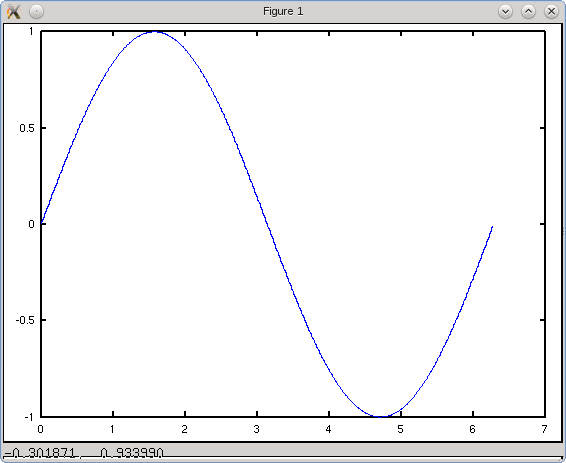
\includegraphics[width=0.4\textwidth]{./octave-plot-sinx}
    \end{center}
    \framebreak
    \item Procedure for plotting 3D graphics
    \begin{enumerate}
      \item Generate a grid data for a 3D plot: Requires two matrices $xx$ whose rows are copies of $x$ and $yy$ whose columns are copies of y
      \begin{verbatim}
octave:1> x = 0:0.1:3*pi;
octave:2> y = 0:0.1:3*pi;
octave:3> [xx,yy]=meshgrid(x,y);
      \end{verbatim}
    \item Plot a surface in 3D
      \begin{verbatim}
octave:4> z = sin(x)'*cos(y);
octave:5> mesh(x,y,z);
      \end{verbatim}
    \end{enumerate}
    \begin{center}
      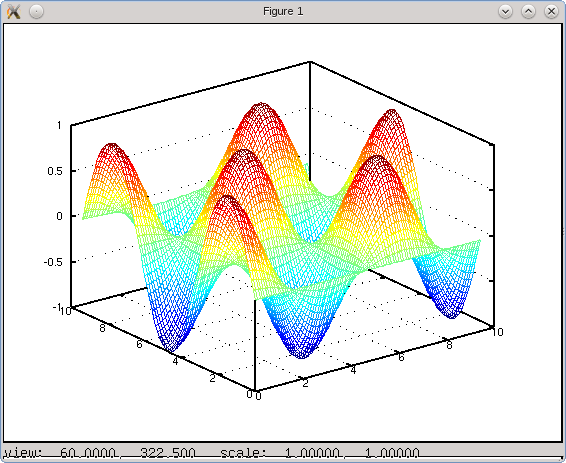
\includegraphics[width=0.35\textwidth]{./octave-plot-3d}
    \end{center}
  \end{itemize}
\end{frame}

\begin{frame}[fragile,allowframebreaks]
  \frametitle{\small Commands for 2D and 3D graphics}
  \begin{itemize}
    \item \texttt{title(string)} writes \texttt{string} as title for the graphics
    \item \texttt{xlabel(string)} labels the $x-$axis with \texttt{string}
    \item \texttt{ylabel(string)} labels the $y-$axis with \texttt{string}
    \item \texttt{zlabel(string)} labels the $z-$axis with \texttt{string}
    \item \texttt{axis(v)} set axes limits for the plot. \texttt{v} is a vector of the form \texttt{v = (xmin,xmax,ymin,ymax[,zmin,zmax])}.
    \item \texttt{hold [on|off]} controls whether the next graphics output should or shouldn't clear the previous graphics.
    \item \texttt{clg} clears the graphics window.
  \end{itemize}
  \framebreak
%octave:1> x = 0:0.1:3*pi;
%octave:2> y = 0:0.1:3*pi;
%octave:3> [xx,yy]=meshgrid(x,y);
%octave:4> z = sin(x)'*cos(y);
%octave:5> mesh(x,y,z);
  \begin{verbatim}
octave:6> title('My 3D Plot');
octave:7> xlabel('x');
octave:8> ylabel('y');
octave:9> zlabel('sin(x)*cos(y)');
  \end{verbatim}
  \begin{center}
    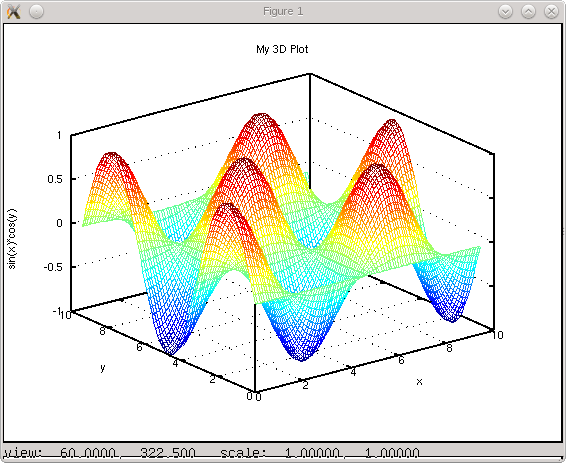
\includegraphics[width=0.5\textwidth]{./octave-plot-3d-title}
  \end{center}
\end{frame}


\section{Loops and Conditions}
\begin{frame}[fragile, allowframebreaks]
  \frametitle{\small Control Statements}
  \begin{itemize}
    \item Control Statements such as \texttt{if, do, while} and so on control the flow of execution in Octave Programs.
    \item Each control statement has an \texttt{end} statement that marks the end of the control statement.
  \end{itemize}
  \begin{eblock}{The IF Statement}
    The general form of the \texttt{IF} statement is
    {\tiny
      \begin{columns}
        \column{4cm}
        \begin{verbatim}
if (condition)
  then-body
elseif (condition)
  elseif-body
else
  else-body
endif
        \end{verbatim}
        \column{6cm}
        \begin{verbatim}
if (rem (x,2) == 0)
    printf (``x is even\n'');
elseif (rem (x,3) == 0)
    printf (``x is odd and divisible by 3\n'');
else
    printf (``x is odd\n'')
endif
        \end{verbatim}
      \end{columns}
    }
    The \texttt{elseif} and \texttt{else} blocks are optional
  \end{eblock}

  \begin{eblock}{The SWITCH Statement}
    The \texttt{SWITCH} statement is similar to the \texttt{SELECT CASE} statement in Fortran 90 and allows one to carry out different operation based on one variable.
    {\tiny
      \begin{columns}
        \column{3cm}
        \begin{verbatim}
switch expression
  case label
    command_list
  case label
    command_list
  otherwise
    command_list
endswitch
        \end{verbatim}
        \column{7cm}
        \begin{verbatim}
a = rem (y,2);
switch a
  case 0
    printf (``x is even\n'');
  otherwise
    b = rem (y,3);
    switch b
      case 0
        printf (``x is odd and divisible by 3\n'');
      otherwise
        printf (``x is odd\n'')
    endswitch
endswitch
        \end{verbatim}
      \end{columns}
    }
  \end{eblock}

  \begin{eblock}{The WHILE Statement}
    The \texttt{WHILE} statement is the simplest form of a looping construct. It repeatedly executes a statement as long as a condition is true
    {\tiny
      \begin{columns}
        \column{4cm}
        \begin{verbatim}
while (condition)
  body
endwhile
        \end{verbatim}
        \column{6cm}
        \begin{verbatim}
fib = ones(1, 10);
i = 3;
while ( i <= 10 )
  fib(i) = fib(i-1) + fib(i-2); 
  i++;
endwhile
        \end{verbatim}
      \end{columns}
    }
  \end{eblock}

  \begin{eblock}{The DO-UNTIL Statement}
    The \texttt{DO-UNTIL} statement is similar to the \texttt{WHILE} statement except that it repeatedly executes a statement until a condition is true. The test of the condition is at the end of the loop so that the loop executes at least once.
    {\tiny
      \begin{columns}
        \column{4cm}
        \begin{verbatim}
do
  body
until (condition)
        \end{verbatim}
        \column{6cm}
        \begin{verbatim}
fib = ones(1, 10);
i = 2;
do
  i++;
  fib(i) = fib(i-1) + fib(i-2) 
until ( i == 10)
        \end{verbatim}
      \end{columns}
    }
  \end{eblock}

  \begin{eblock}{The FOR Statement}
    The \texttt{FOR} statement makes it convenient to count iterations of a loop
    {\tiny
      \begin{columns}
        \column{3cm}
        \begin{verbatim}
for var = expression
  body
endfor
        \end{verbatim}
        \column{7cm}
        \begin{verbatim}
for I=1:N
  sumft=0;
  for J=1:M
    sumft=sumft+ftmwvels(I,J)^2;
  endfor
  fprintf(fid,'' %15.8e  %21.14e\n'',(I-1)*dw,sumft);
endfor
        \end{verbatim}
      \end{columns}
    }
  \end{eblock}

  \begin{eblock}{The BREAK and CONTINUE Statements}
    \begin{itemize}
      \item[] The \texttt{BREAK} statement allows you to jump from the inside of a loop past the end of a loop
      \item[] The \texttt{CONTINUE} statement allows you to jump from the inside of a loop to the beginnng of the loop
      \item[] The \texttt{BREAK} and \texttt{CONTINUE} can be used inside a \texttt{for, while} or \texttt{do$\dots$until} loop.
    \end{itemize}
    {\tiny
%      \begin{columns}
%        \column{5cm}
        \begin{verbatim}
total = 0;
while true
   x = input('Value to add (enter 0 to stop): ');
   if x == 0
      break;
   endif
   total = total+x;
   disp(['Total: ', num2str(total)]);
endwhile

N = 5;
A = zeros(N); % Create an N x N matrix filled with 0s

for row = 1:N
   for column = 1:N
      if column > row
         continue;
      endif
      A(row, column) = 1;
   endfor
endfor
        \end{verbatim}
%      \end{columns}
    }
  \end{eblock}
\end{frame}

\section{File I/O}
\begin{frame}[fragile,allowframebreaks]
  \frametitle{\small Simple File I/O}
  \begin{itemize}
    \item \texttt{save} and \texttt{load} commands allow data to be written to and read from disk files in various formats.
    {\tiny
      \begin{verbatim}
apacheco-3:~ apacheco> octave -q
octave-3.2.3:1> A = [1 2 3; 4 5 6; 7 8 9];
octave-3.2.3:2> save myfile.mat A
octave-3.2.3:3> 
apacheco-3:~ apacheco> cat myfile.mat 
# Created by Octave 3.2.3, Fri Apr 13 12:53:36 2012 CDT <apacheco@apacheco-3.lsu.edu>
# name: A
# type: matrix
# rows: 3
# columns: 3
 1 2 3
 4 5 6
 7 8 9
apacheco-3:~ apacheco> octave -q
octave-3.2.3:1> load myfile.mat
octave-3.2.3:2> A
A =

   1   2   3
   4   5   6
   7   8   9
      \end{verbatim}
    }
    \item Octave can save and read data in various formats such as ASCII, binary, MATLAB binary format, hdf5.
  \end{itemize}
\end{frame}

\begin{frame}[fragile]
  \frametitle{\small C style I/O Functions}
  \begin{itemize}
    \item Octave C style input and output functions provides most of the functionality of C programming language's standard I/O library.
    \item Opening and Closing Files: When reading or writing data to a file, it must be opened first
    {\tiny
      \begin{verbatim}
fid = fopen(``water-hexamer-cage-bomd.ftmwvels'',''w'');
dw = 1/(N*deltat);
for I=[1:N]
  sumft=0;
  for J=[1:M]
    sumft=sumft+ftmwvels(I,J)^2;
  endfor
  fprintf(fid,'' %15.8e  %21.14e\n'',(I-1)*dw,sumft);
endfor
fclose(fid);
      \end{verbatim}
    }
    \item Octave can open files in various modes, the above example is for writing.
    \begin{description}
      \item[r]: Open a file for reading.
      \item[w]: Open a file for writing.
      \item[a]: Open or create a file for writing at the end of the file.
      \item[r+]: Open an existing file for reading and writing.
      \item[w+]: Open a file for reading and writing and discard previous contents.
      \item[a+]: Open or create a file for reading and writing at the end of the file.
    \end{description}
  \end{itemize}
\end{frame}

\begin{frame}[fragile]
  \frametitle{\small Formatted Output}
  \begin{itemize}
    \item Octave provides function for printed formatted output which are modelled on the C language functions.
    \begin{description}
      \item[printf (template, $\dots$)]: Print optional argumentsunder the control of string \texttt{template}.
      \item[fprintf (fid, template, $\dots$)]: Same as \texttt{printf} except that output is written to stream \texttt{fid} instead of \texttt{stdout}.
      \item[sprintf (template, $\dots$)]: Same as \texttt{printf} except that the output is returned as a string.
    \end{description}
    \item Output Conversion Syntax:
    \item[] General Form: \texttt{\% flags width [.precision] type conversion}
    \begin{description}
      \item[\%7d]: Prints an integer with a width of 7.
      \item[\%8.3f]: Prints a floating point number with a width of 8 and precision of 3.
      \item[\%11s]: Prints a string of width 11.
      \item[\%21.14e]: Prints a floating point number in exponential notation with a width of 21 and precision 14.
    \end{description}
  \end{itemize}
\end{frame}

\section{Functions}
\begin{frame}[fragile,allowframebreaks]
  \frametitle{\small Functions}
  \begin{itemize}
    \item Complicated Octave programs can be simplified by defining functions.
    \item In the simplest form, a function, \texttt{name}, is defined as follows:
   {\tiny
     \begin{columns}
       \column{4cm}
       \begin{verbatim}
function name (argument-list)
   body
endfunction
       \end{verbatim}
       \column{4cm}
       \begin{verbatim}
[apacheco@tezpur1 octave]$ cat hello.m 
function hello (message)
   printf (``%s\n'',message)                                                     
endfunction
[apacheco@tezpur1 octave]$ octave -q
octave:1> hello (``Hello World'')
Hello World
       \end{verbatim}
     \end{columns}
   }
   \item In some instances, your program may need some information back from the function that you have defined.
   \item Syntax for writing a function that returns
   \begin{enumerate}
     \item a single value
     {\tiny
       \begin{verbatim}
function ret-var = name (argument-list)
  body
endfunction
       \end{verbatim}
     }
     \item multiple values
       {\tiny
       \begin{verbatim}
function [ret-list] = name (argument-list)
  body
endfunction
       \end{verbatim}
       }
   \end{enumerate}
   \item The symbol \texttt{ret-var} is the name of the variable that will hold the value to be returned by the function.
   \item The symbol \texttt{ret-list} is a comma separated list of variables that will hold the values returned by the function.
   \item \texttt{ret-var} and \texttt{ret-list} must be defined before the end of the function body.
   \item Variables defined in the function including \texttt{ret-var, ret-list} and \texttt{argument-list} are local to the function.
   {\tiny
     \begin{columns}
       \column{4cm}
       \begin{verbatim}
v = rand(10,1);

function average = avg (a)
  average = sum(a)/length(a) ;
endfunction

function [max,id] = vmax(a)
  id = 1;
  max = a(id);
  for i = 2:length(a)
    if ( a(i) > max )
      max = a(i) ;
      id = i ;
    endif
  endfor
endfunction
       \end{verbatim}
       \column{6cm}
       \begin{verbatim}
b = rand(20,1);
[max,id] = vmax(b); 
printf ( ``Average of vector v = %f\n'', avg(v)) 
printf ( ``Maximum value of vector b = %f with \
   id = %d\n'',max,id )


[apacheco@tezpur1 octave] ./func.sh 
Average of vector v = 0.512198
Maximum value of vector b = 0.996040 with id = 7
       \end{verbatim}
     \end{columns}
   }
   \item Instead of defining functions each time you need them, you can save the function to a Function File and use them whenever needed.
   \item Function Files end with a \texttt{.m} extension with a prefix that matches the function name.
   \item Function files should contain only one function, see \texttt{hello.m} two slides back.
   \item When a function is called, octave searches a list of directory for a file that contains the function declaration.
   \item If the function file is not in the current directory, you can add the directory to search for the function file using the \texttt{addpath} command
   \item[] \texttt{addpath("$\sim$/Octave:$\sim$/Octave-Func")}: Add \texttt{$\sim$/Octave} and \texttt{$\sim$/Octave-Func} to the load path for searching function files.
  \end{itemize}
\end{frame}

\section{Scripting}
\begin{frame}[fragile,allowframebreaks]
  \frametitle{\small Script Files}
  \begin{itemize}
    \item A script file is a file containing any sequence of Octave commands.
    \item It is read and evaluated as if you have entered the commands interactively at the octave prompt.
    \item A script file must not begin with a function keyword. If the script file begins with a function keyword, Octave will assume that it is a function file and will evaluate only the function when it is called.
    \item Unlike a function file, variables in the script file are global and can be accessed by any line/command in the script.
    \item Octave normally executes commands from a script file with a \texttt{.m} extension.
    \item The \texttt{source} command allows Octave to execute commands from any file
    \item[] \texttt{source(file.exe)} to execute commands in the \texttt{file.exe} file.
    {\tiny
      \begin{verbatim}
[apacheco@tezpur1 octave]$ cat func.txt
v = rand(10,1);

function average = avg (a)
  average = sum(a)/length(a) ;
endfunction

function [max,id] = vmax(a)
  id = 1;
  max = a(id);
  for i = 2:length(a)
    if ( a(i) > max )
      max = a(i) ;
      id = i ;
    endif
  endfor
endfunction

b = rand(20,1);
[max,id] = vmax(b); 

printf ( ``Average of vector v = %f\n'', avg(v)) 
printf ( ``Maximum value of vector b = %f with id = %d\n'',max,id )

[apacheco@tezpur1 octave]$ octave -q
octave:1> source('func.txt')
Average of vector v = 0.487381
Maximum value of vector b = 0.878363 with id = 14
      \end{verbatim}
    }
    \item Octave also allows you to create an executable script file.
    \item The first line of the executable script file should refer the interpreter.
    \item Octave Executable scripts can take command line arguments.
    \item The built-in function \texttt{argv} returns a cell array containing the command line arguments passed to the executable script.
    \item The built-in function \texttt{nargin} returns the number of arguments passed.
    \item On Tezpur, first line should be
    \item[]{\tiny\texttt{\#!/usr/local/packages/octave/3.0.3/intel-11.1/bin/octave -qf}}
    {\tiny
      \begin{verbatim}
[apacheco@tezpur1 octave]$ cat func.sh 
#!/usr/local/packages/octave/3.0.3/intel-11.1/bin/octave -qf

v = rand(10,1);

function average = avg (a)
  average = sum(a)/length(a) ;
endfunction

function [max,id] = vmax(a)
  id = 1;
  max = a(id);
  for i = 2:length(a)
    if ( a(i) > max )
      max = a(i) ;
      id = i ;
    endif
  endfor
endfunction

b = rand(20,1);
[max,id] = vmax(b); 

printf ( ``Average of vector v = %f\n'', avg(v)) 
printf ( ``Maximum value of vector b = %f with id = %d\n'',max,id )

[apacheco@tezpur1 octave]$ ls -l func.sh 
-rwxr-xr-x  1 apacheco Admins 450 Apr 16 11:39 func.sh
[apacheco@tezpur1 octave]$ ./func.sh 
Average of vector v = 0.599684
Maximum value of vector b = 0.986472 with id = 15
      \end{verbatim}
    }
  \end{itemize}
\end{frame}

\begin{frame}[fragile,allowframebreaks]
  \frametitle{\small Calculate Spectra from AIMD Simulation}
  \begin{itemize}
    \item Octave script to calculate Fourier Transform of Auto-Correlation Function of Mass Weighted Velocities. /home/apacheco/octave-tutorial/getftmwvels.sh
  {\tiny
    \begin{verbatim}
[apacheco@tezpur1 octave-tutorial]$ cat getftmwvels.sh
#!/usr/local/packages/octave/3.0.3/intel-11.1/bin/octave -qf

if(nargin!=4)
   printf (``%s\n'', ``This script needs 4 arguments, [Velocity File (input)], \
        [FT-VAC File (output)], [Number of Atoms], [Time Step in fs]'' )
endif

arg_list = argv();
printf (``Argument list:'');
for i = 1:nargin
  printf (`` %s'', arg_list{i});
endfor
printf (``\n'');

Vels = arg_list{1};
VelsFT = arg_list{2};
NAtoms = eval(arg_list{3});
deltat = eval(arg_list{4});

M = NAtoms*3;
mwvels = load(Vels);
N = rows(mwvels);
ftmwvels = abs(fft(mwvels,N));
fid = fopen(VelsFT,''w'');

dw = 1/(N*deltat);
for I=[1:N]
  sumft=0;
  for J=[1:M]
    sumft=sumft+ftmwvels(I,J)^2;
  endfor
  fprintf(fid,'' %15.8e  %21.14e\n'',(I-1)*dw,sumft);
endfor
fclose(fid);

# Below was added for octave tutorial
A=load(VelsFT);
int=A(:,1)*33356; # convert from fs^-1 to cm^-1
spectra_orig=A(:,2)/norm(A(:,2)); # normalized original spectra
# Do interpolation of Spectra for octave demo
intensity=linspace(0,4000,400000);
# Linear Interpolation
spectra_lin=interp1(int,spectra_orig,intensity,'linear');
# Spline Interpolation
spectra_spl=interp1(int,spectra_orig,intensity,'spline');
# Cubic Interpolation
spectra_cub=interp1(int,spectra_orig,intensity,'cubic');

plot(int,spectra_orig,'r',intensity,spectra_lin+0.2,'g', \
  intensity,spectra_spl+0.4,'b',intensity,spectra_cub+0.6,'m');

legend("original","linear","spline","cubic");
axis([0,4000,0,1]);
xlabel('Intensity');
ylabel('Normalized Spectra');

print -deps spectra.eps;
    \end{verbatim}
  }
  \item Usage: 
  {\tiny
    \begin{verbatim}
[apacheco@tezpur1 water-hexamer]$ ./getftmwvels.sh water-hexamer-cage-admp.mwvels \
> water-hexamer-cage-admp.ftmwvels 18 0.25
Argument list: water-hexamer-cage-admp.mwvels water-hexamer-cage-admp.ftmwvels 18 0.25

[apacheco@tezpur1 water-hexamer]$
    \end{verbatim}
  }
  \end{itemize}
  \begin{center}
    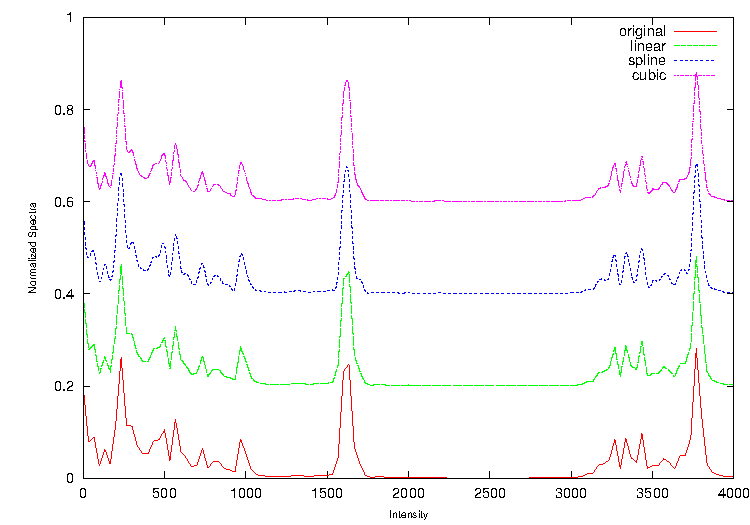
\includegraphics[width=0.8\textwidth]{./spectra}
  \end{center}
\end{frame}

\begin{frame}
  \frametitle{\small References}
  \begin{enumerate}
    \item Octave Manual: \url{http://www.gnu.org/software/octave/doc/interpreter/index.html} and \url{http://www.gnu.org/software/octave/octave.pdf}
    \item Octave-Forge: \url{http://octave.sourceforge.net/}
    \item Octave Tutorials: \url{http://en.wikibooks.org/wiki/Octave_Programming_Tutorial}
  \end{enumerate}
\end{frame}
\end{document}
